\chapter{System Design}

\section{Introduction}

Following the requirements analysis presented in the previous chapter, this chapter focuses on the design of the proposed system. The objective of this phase is to translate the identified functional and non-functional requirements into a coherent and structured system architecture that ensures scalability, maintainability, and efficient interaction between components.

The system design is centered around a multi-channel architecture in which WhatsApp serves as the primary interaction interface for farmers, while a web application provides structured management environments for agronomists and administrators. Both channels are supported by a backend infrastructure responsible for data management, request processing, and integration with external services. The design adopts a modular approach, allowing the separation of concerns between the interaction layer, the orchestration logic, the agent layer, and the data layer.

In this chapter, we first present the overall system architecture, highlighting the different components and their interactions. We then introduce the multi-agent system perspective adopted in the design, followed by a set of UML models that describe the system from functional and structural viewpoints. Subsequently, we detail the workflow design, database structure, and data modeling choices that support the application's functionality.

Finally, we discuss the orchestration strategy as well as the mechanisms for context management and personalization, which aim to enhance user experience and system adaptability. This comprehensive design provides a solid foundation for the implementation phase presented in the next chapter.

\section{Overall System Architecture}

AgriConnect is built on a five-layer architecture designed to support multimodal farmer interaction, intelligent multi-agent reasoning, and collaborative case management between farmers, agronomists, and administrators. Each layer has a clearly defined responsibility, and the layers communicate through well-defined data flows, external calls, and event-driven triggers. Figure~\ref{fig:architecture} provides a global view of the system and the relationships between its components.

\begin{figure}[H]
    \centering
    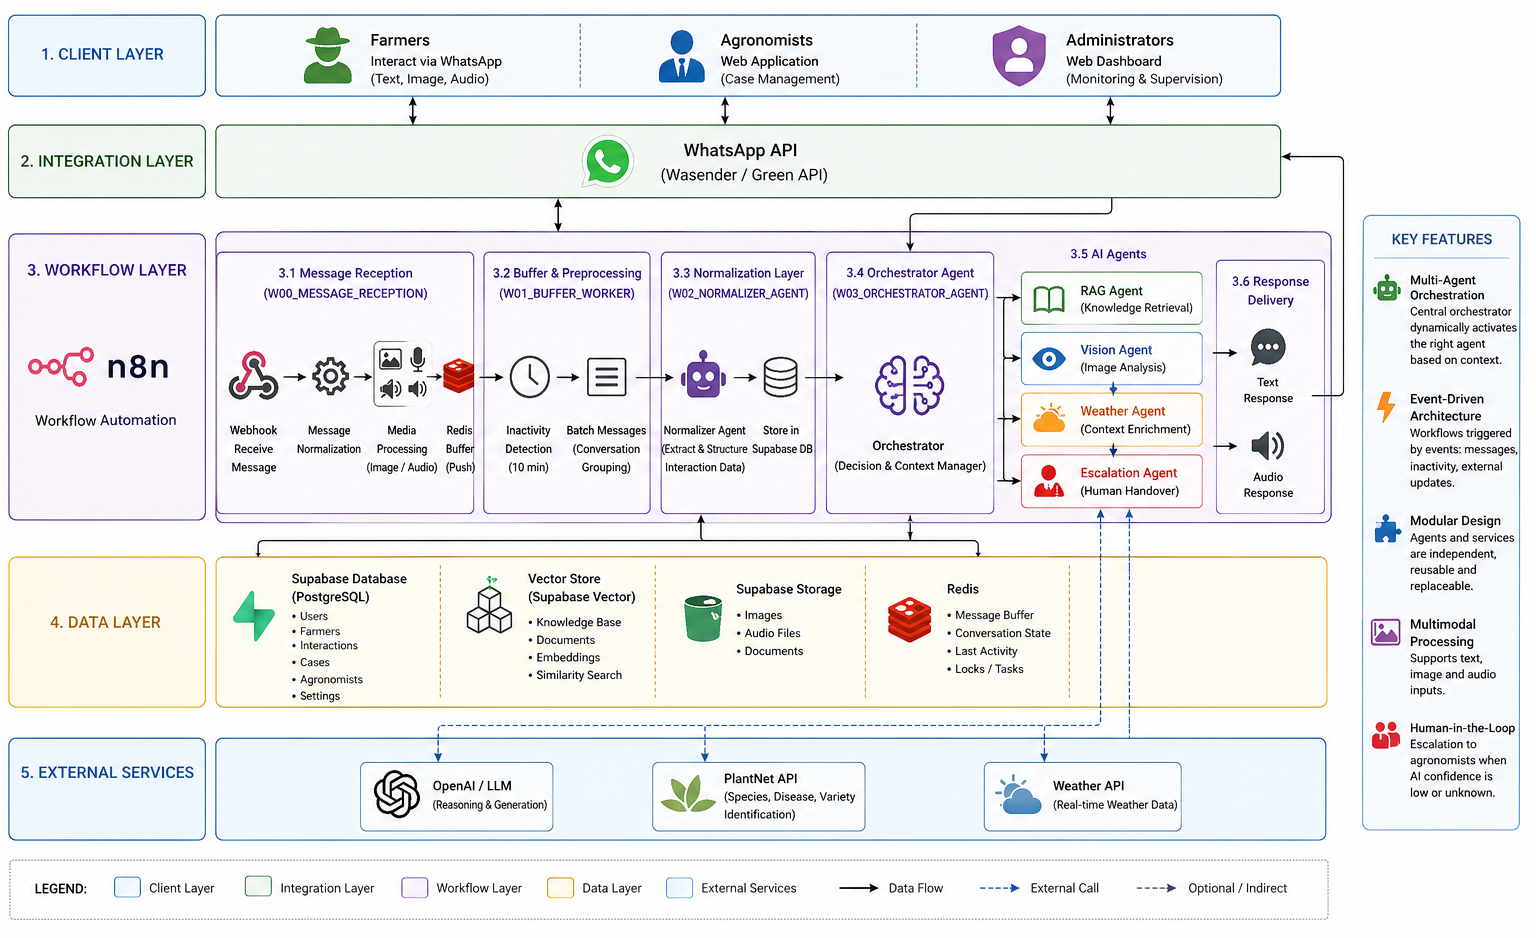
\includegraphics[width=\textwidth]{images/diagrammes/system_architecture.png}
    \caption{Overall System Architecture of AgriConnect}
    \label{fig:architecture}
\end{figure}

\subsection*{Layer 1 — Client Layer}

The client layer defines the three categories of users and the interfaces through which they interact with the platform. Farmers communicate exclusively through WhatsApp, sending text messages, images of crops, and audio notes in a natural and low-barrier manner. Agronomists access a dedicated web application designed for case management, where they can review pending cases, submit proposals, and follow intervention history. Administrators use a web dashboard that provides monitoring and supervision capabilities, including user management, knowledge base maintenance, and platform-wide statistics.

\subsection*{Layer 2 — Integration Layer}

The integration layer provides the communication bridge between the client layer and the internal system. All WhatsApp interactions are routed through the WhatsApp Business API, connected via Wasender and Green API. This layer is responsible for receiving incoming messages from farmers and delivering outgoing responses back to the same channel. The bidirectional nature of this layer ensures that the platform can maintain a continuous and responsive communication loop with farmers through their preferred messaging application.

\subsection*{Layer 3 — Workflow Layer}

The workflow layer constitutes the operational core of the system. It is implemented using n8n, an event-driven workflow automation engine, and is composed of four distinct workflows: a message reception workflow, a main orchestration workflow, a vision analysis sub-workflow, and a knowledge base ingestion workflow.

\textbf{W00 — Message Reception} is triggered by an incoming webhook from the WhatsApp API via Wasender. The raw payload is normalized into a structured internal format, and the sender's phone number is verified against the Supabase farmer registry. If the farmer is not registered, the system automatically replies with an invitation to create an account. If registered, the message is routed by content type. Text messages pass through a guardrails safety check before being admitted. Audio messages are decrypted via the Wasender API, downloaded, and transcribed into text using the OpenAI Whisper model. Image messages are decrypted, downloaded, and stored in Supabase Storage. In all admitted cases, the processed message is pushed onto a Redis buffer list identified by the sender's phone number, and a Redis key tracking last activity is updated with a fifteen-minute TTL.

\textbf{W01 — Orchestrator Workflow} is a single workflow that internally handles all stages from buffer processing to response delivery. It is triggered by a scheduled timer running every five seconds, which scans active Redis buffer keys and checks whether each buffer's inactivity key has expired. Once a buffer is considered complete, its messages are extracted, grouped into a batch, and classified as text-only or image-inclusive. When an image is present, a visual preanalysis step is executed: a signed URL is generated for the stored image, the image is downloaded, and a local vision model (Ollama/LLaVA) produces factual visual observations. A structured preanalysis object is built from these observations, covering agriculture-relatedness, image quality, and preliminary hypotheses. If this step fails, a safe default preanalysis is used to ensure continuity. The batch and preanalysis are then passed to the Normalizer Agent, an LLM-based agent (GPT-4o-mini) that extracts a structured representation including the farmer's main question in English, detected crops, symptoms, urgency signals, and location hints. A Structured Output Parser enforces a strict JSON schema on the output. The normalized batch is persisted in Supabase and the Redis buffer is cleared. The Orchestrator Agent (GPT-4.1-mini) then receives the normalized inputs, retrieves the farmer profile and recent interaction history from Supabase, and consults a PostgreSQL-backed conversation memory to maintain context across turns. Based on this enriched context, it selectively invokes four specialized sub-agents: the \textit{RAG Agent} for knowledge base retrieval using OpenAI embeddings over the Supabase vector store; the \textit{Vision Agent} for deep image analysis via the dedicated Vision sub-workflow; the \textit{Weather Agent} for real-time meteorological context using OpenWeatherMap; and the \textit{Escalation Agent} for creating formal agronomist cases in the database. Finally, the orchestrator's structured output is extracted and routed based on the \texttt{response\_format} field: text responses are sent directly via the WhatsApp API, while audio responses are generated using the OpenAI TTS model, uploaded to Supabase Storage, and delivered as a WhatsApp audio message through a temporary signed URL.

\textbf{Vision Sub-Workflow} is a dedicated workflow called as a tool by the Orchestrator Agent when a crop image is eligible for deep analysis. It receives the image URL, vision observations, and farmer question as inputs. The image is downloaded in parallel and submitted to four complementary PlantNet API endpoints: a general species identification endpoint (\texttt{/all}), a targeted flora identification endpoint (\texttt{/k-world-flora}), a disease detection endpoint (\texttt{/diseases/identify}), and a variety identification endpoint (\texttt{/varieties/identify}). The results of all four calls are merged and normalized into a single structured output containing ranked species candidates, disease candidates, variety candidates, quality issues, and a recommended next step, which is returned to the orchestrator.

\textbf{KB Ingestion Workflow} is an independent workflow responsible for maintaining the agricultural knowledge base. It is triggered automatically by a Google Drive event whenever a new document is added to the designated knowledge base folder. Upon trigger, the file metadata is extracted and deduplicated, any existing document chunks associated with the same file identifier are deleted from the Supabase vector store to avoid duplication, and the new file is downloaded from Google Drive, loaded using a DOCX document loader, chunked, and embedded using the OpenAI embedding model before being upserted into the Supabase vector store. An email notification is then sent to the administrator confirming the successful ingestion of the new document.

\subsection*{Layer 4 — Data Layer}

The data layer provides persistent storage for all structured and unstructured data managed by the system. It is composed of four components. The \textbf{Supabase PostgreSQL} database stores all core relational data including users, farmers, agronomists, interactions, cases, and platform settings. The \textbf{Supabase Vector Store} supports the RAG agent by indexing embedded document chunks and enabling similarity-based retrieval across the agricultural knowledge base. \textbf{Supabase Storage} handles binary assets such as images, audio files, and documents uploaded during interactions or case creation. Finally, \textbf{Redis} serves as an in-memory store for message buffering, conversation state, last activity timestamps, and workflow-level locks and tasks.

\subsection*{Layer 5 — External Services}

The external services layer groups the third-party APIs that extend the system's capabilities beyond its internal logic. \textbf{OpenAI / LLM} provides the reasoning and natural language generation capabilities used by multiple agents across the workflow. The \textbf{PlantNet API} enables visual plant identification by returning species, disease, and variety candidates from crop images submitted by farmers. The \textbf{Weather API} supplies real-time meteorological data used by the weather agent to contextualize agronomic recommendations according to local conditions.

\vspace{0.5cm}

This five-layer design ensures a clear separation of concerns across the platform. The event-driven architecture of the workflow layer allows each component to react to incoming signals independently, while the modular structure of the agent layer ensures that agents remain independently deployable and replaceable. Together, these design principles support the accessibility, reliability, modularity, and extensibility requirements identified during the analysis phase.

\section{Multi-Agent System Design}

AgriConnect is designed as a multi-agent system in which a central orchestrator coordinates a set of specialized agents, each responsible for a distinct cognitive or operational function. This design reflects a deliberate separation between the reasoning about what to do and the execution of specific capabilities, which improves modularity, traceability, and the ability to update individual agents without affecting the overall pipeline.

The \textbf{Orchestrator Agent} is the central decision-making component. It receives a normalized representation of the farmer's interaction, loads contextual information from the farmer profile and interaction history, and determines which specialized agents to invoke based on the content, intent, and urgency of the request. It is responsible for fusing the outputs of all activated agents and producing a final coherent response.

The \textbf{RAG Agent} is responsible for knowledge-grounded response generation. When agronomic documentation is required, it queries the Supabase vector store using semantic embeddings to retrieve the most relevant knowledge base passages. Its responses are strictly limited to retrieved evidence to minimize hallucination risk.

The \textbf{Vision Agent} is a sub-workflow agent dedicated to deep crop image analysis. It is invoked only when the incoming message contains an image that passes a quality and agriculture-relatedness preanalysis. It submits the image to four complementary PlantNet API endpoints in parallel and returns a structured ensemble result covering species, disease, and variety candidates.

The \textbf{Weather Agent} enriches agronomic recommendations with environmental context. It resolves the farmer's geographical location, queries a weather API for current conditions and short-term forecasts, and returns agronomic signals such as heat stress risk, fungal risk window, and spraying conditions.

The \textbf{Escalation Agent} handles situations that exceed the system's automated reasoning capacity. When the orchestrator identifies a case as urgent, unresolved, or requiring professional expertise, the Escalation Agent creates a formal case record in the database and attaches relevant images, making the case immediately available to an agronomist through the web application.

This architecture supports a human-in-the-loop design principle: the system attempts automated resolution first and escalates to human experts only when the evidence is insufficient or the situation is critical. Each agent operates under strict output contracts enforced by structured JSON schemas, ensuring that the orchestrator always receives predictable and well-formed inputs regardless of which agents were activated.

\section{UML Modeling}
\subsection{Use Case Diagram}

The use case diagram presented in Figure~\ref{fig:usecase} illustrates the functional interactions between the different actors and the AgriConnect system. It provides a high-level view of the system’s functionalities and highlights the roles and responsibilities of each actor.

\begin{figure}[H]
    \centering
    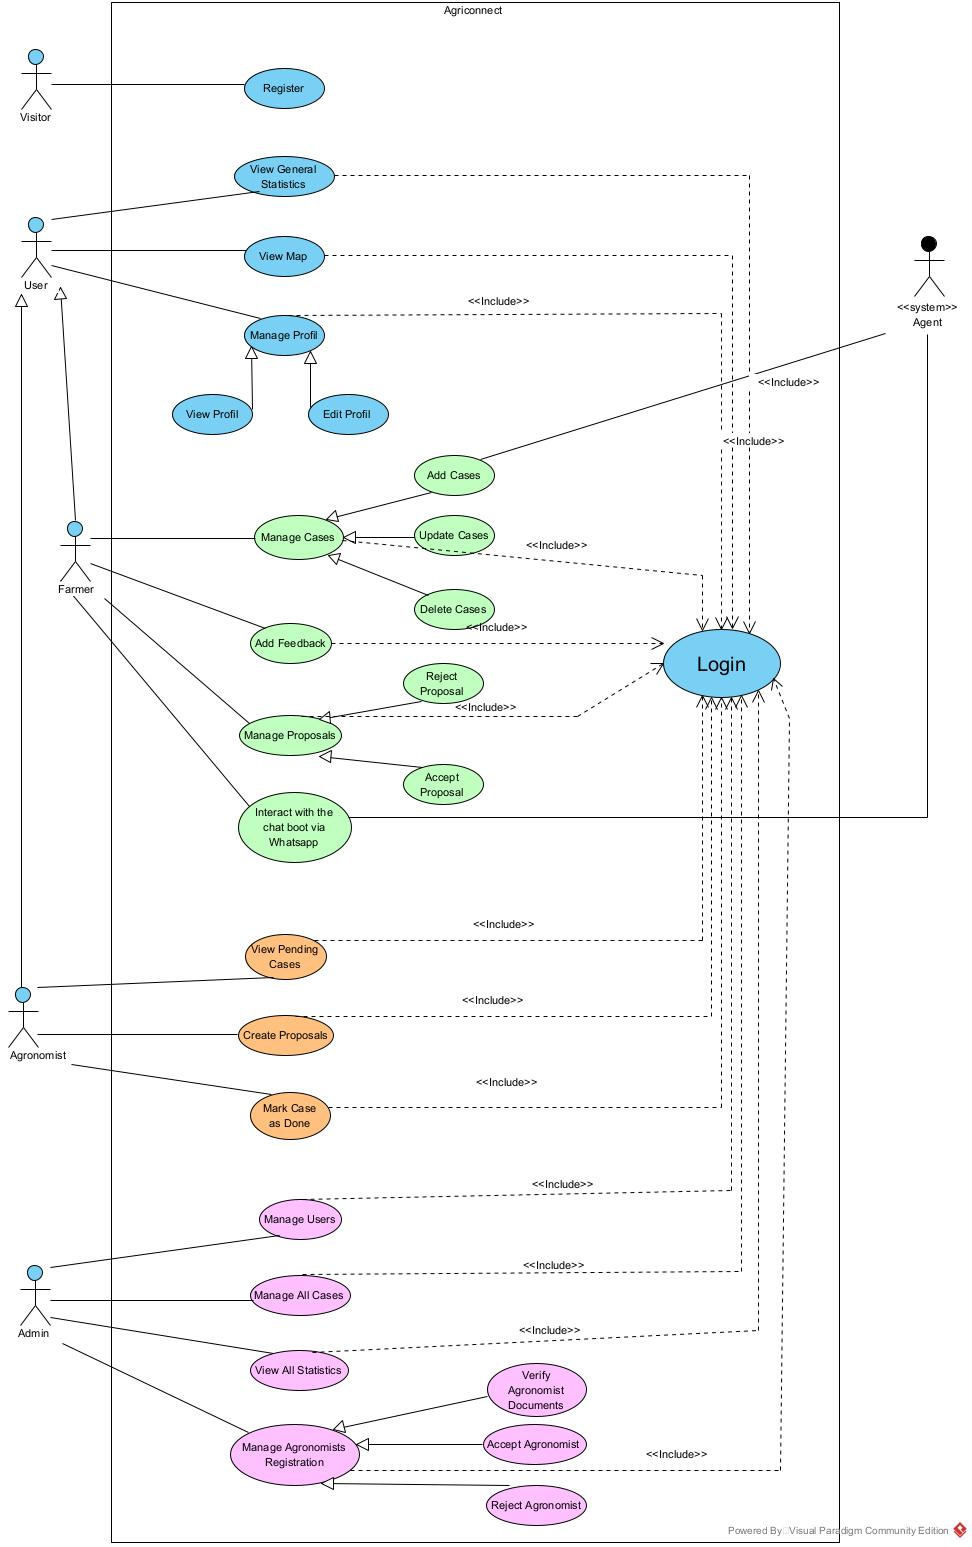
\includegraphics[width=0.95\linewidth]{images/diagrammes/use_case_diagramme_agriconnect.jpeg}
    \caption{AgriConnect Use Case Diagram}
    \label{fig:usecase}
\end{figure}

The system involves multiple actors, each interacting with the platform according to their specific roles. The main actors identified are \textit{Visitor}, \textit{User}, \textit{Farmer}, \textit{Agronomist}, \textit{Admin}, and a \textit{System Agent} representing automated backend processes.

A visitor can register to access the platform, after which they become a user. Authenticated users can manage their profiles by viewing and editing their personal information, as well as access general features such as viewing statistics and maps.

The farmer represents the primary actor of the system. Farmers can manage agricultural cases by creating, updating, and deleting them. They can also interact with agronomists through proposal management, where they can accept or reject proposed solutions. Additionally, farmers can provide feedback and interact with the system via WhatsApp, enabling a more accessible communication channel.

Agronomists play a key role in providing expertise. They can view pending cases submitted by farmers, create proposals, and mark cases as resolved once appropriate solutions are applied.

The administrator is responsible for system supervision and management. This includes managing users, overseeing all cases, viewing global statistics, and handling agronomist registrations through verification, acceptance, or rejection processes.

It is important to note that most functionalities depend on authentication, as indicated by the \textit{<<include>>} relationship with the login use case. This ensures that access to system features is restricted to authorized users.

Overall, this diagram reflects a multi-role system where interactions are structured around case management, collaboration between farmers and agronomists, and administrative control.
\subsection{Class Diagram}

The class diagram illustrated in Figure~\ref{fig:classdiagram} represents the static structure of the AgriConnect system. It models the main entities of the application, their attributes, and the relationships between them, providing a clear view of the system's data organization and object-oriented design.

\begin{figure}[H]
    \centering
    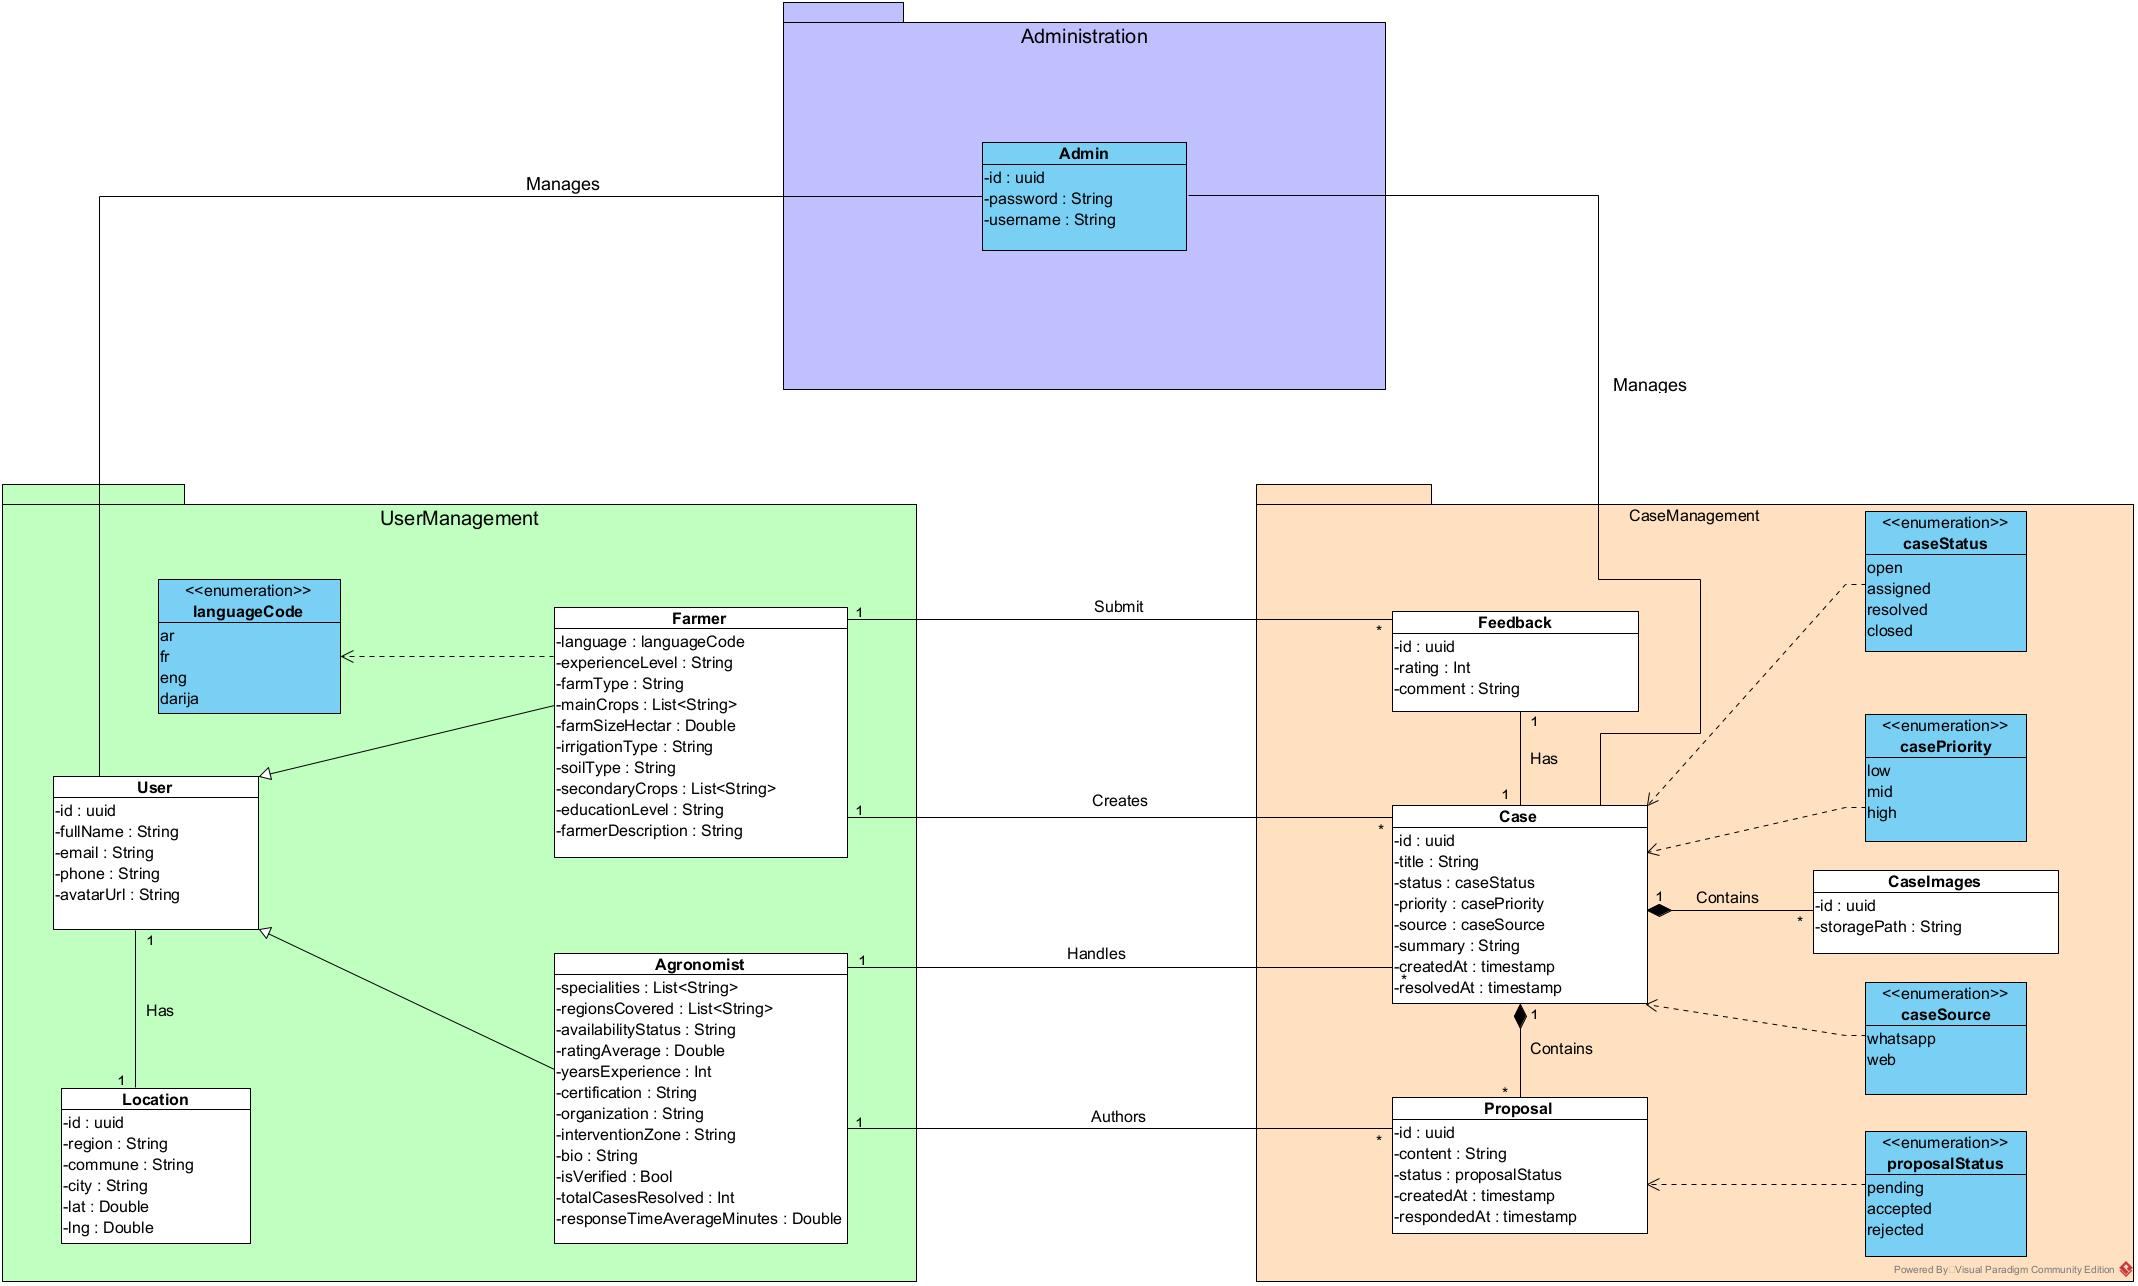
\includegraphics[width=\textwidth]{images/diagrammes/Class_Agriconnect.jpg}
    \caption{AgriConnect Class Diagram}
    \label{fig:classdiagram}
\end{figure}

The system is structured around three main domains: user management, case management, and administration.

The user management domain includes the \textit{User} class, which represents the base entity containing general user information such as identifier, name, email, and contact details. This class is extended by two specialized roles: \textit{Farmer} and \textit{Agronomist}. The farmer class contains domain-specific attributes such as farm characteristics, crop information, and experience level. In contrast, the agronomist class focuses on professional expertise, including specializations, regions covered, certifications, and performance indicators. Additionally, each user is associated with a \textit{Location}, representing geographical information, and a language preference defined by the \textit{languageCode} enumeration.

The case management domain represents the core functionality of the system. The \textit{Case} class models agricultural issues submitted by farmers, including attributes such as title, status, priority, and timestamps. A farmer can create multiple cases, while an agronomist is responsible for handling them. Each case can contain multiple \textit{Proposal} instances, which represent solutions or recommendations provided by agronomists. These proposals have their own lifecycle, defined by the \textit{proposalStatus} enumeration. Furthermore, a case may include associated \textit{CaseImages} for visual context and \textit{Feedback} provided by farmers after resolution.

Several enumerations are used to standardize system states and attributes, including \textit{caseStatus}, \textit{casePriority}, and \textit{caseSource}, ensuring consistency and clarity in the management of cases.

The administration domain is represented by the \textit{Admin} class, which is responsible for overseeing system operations, including user and case management. This role ensures proper governance and control within the platform.

Overall, this class diagram reflects a modular and extensible design, where responsibilities are clearly separated, and relationships between entities are well defined to support the system’s core functionalities.

\subsection{State Machine Diagram}

The state machine diagram presented in Figure~\ref{fig:statediagram} illustrates the lifecycle of a case within the AgriConnect system. It describes the different states a case can go through, as well as the transitions triggered by user actions and system events.

\begin{figure}[H]
    \centering
    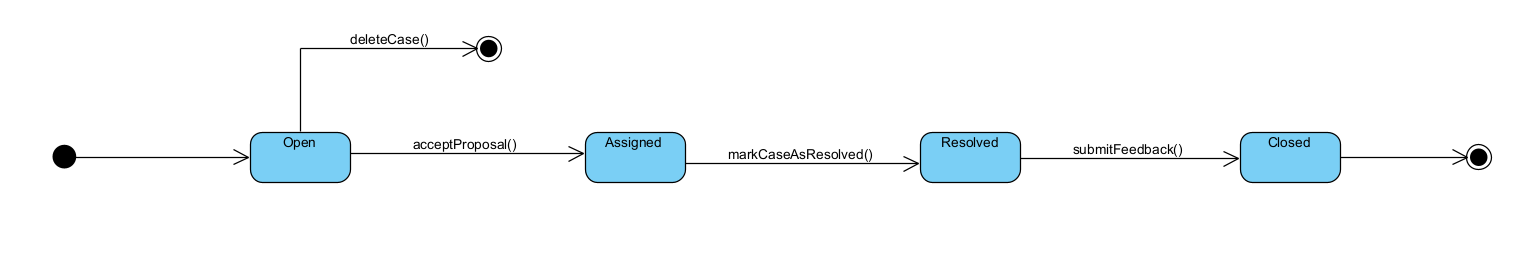
\includegraphics[width=\textwidth]{images/diagrammes/stateMachine_Case_Agriconnect.jpg}
    \caption{Case Lifecycle State Machine Diagram}
    \label{fig:statediagram}
\end{figure}

A case is initially created in the \textit{Open} state, where it is available for review by agronomists. At this stage, the farmer has submitted a problem but no solution has yet been assigned.

When an agronomist submits a proposal and the farmer accepts it, the case transitions to the \textit{Assigned} state. This indicates that a solution is being actively handled.

Once the agronomist applies the solution or marks the issue as resolved, the case moves to the \textit{Resolved} state. At this point, the problem is considered technically solved, but the process is not yet fully completed.

The case reaches the final \textit{Closed} state after the farmer submits feedback, confirming the resolution and completing the interaction cycle.

Additionally, the diagram shows that a case can be deleted directly from the \textit{Open} state, representing an early termination scenario before any processing occurs.

This state machine ensures a clear and controlled progression of cases, improving traceability, consistency, and overall management of agricultural issues within the system.

\section{Workflow Design}

The AgriConnect platform is implemented as four coordinated n8n workflows, each responsible for a distinct processing scope. The architecture is entirely event-driven: workflows are triggered by incoming WhatsApp messages, scheduled timers, Redis state changes, or Google Drive events. Together, these four workflows form a pipeline that transforms raw farmer messages into structured, grounded, and personalized responses, while also maintaining the agricultural knowledge base independently.

\subsection{W00 — Message Reception Workflow}

W00 is the entry point of the system, triggered by an incoming WhatsApp webhook. It normalizes the raw payload, verifies farmer registration, routes the message by type (text through guardrails, audio through Whisper transcription, image through Supabase Storage upload), and pushes the result onto a Redis buffer with an inactivity TTL. The full step-by-step implementation is detailed in the realization chapter.

\begin{figure}[H]
    \centering
    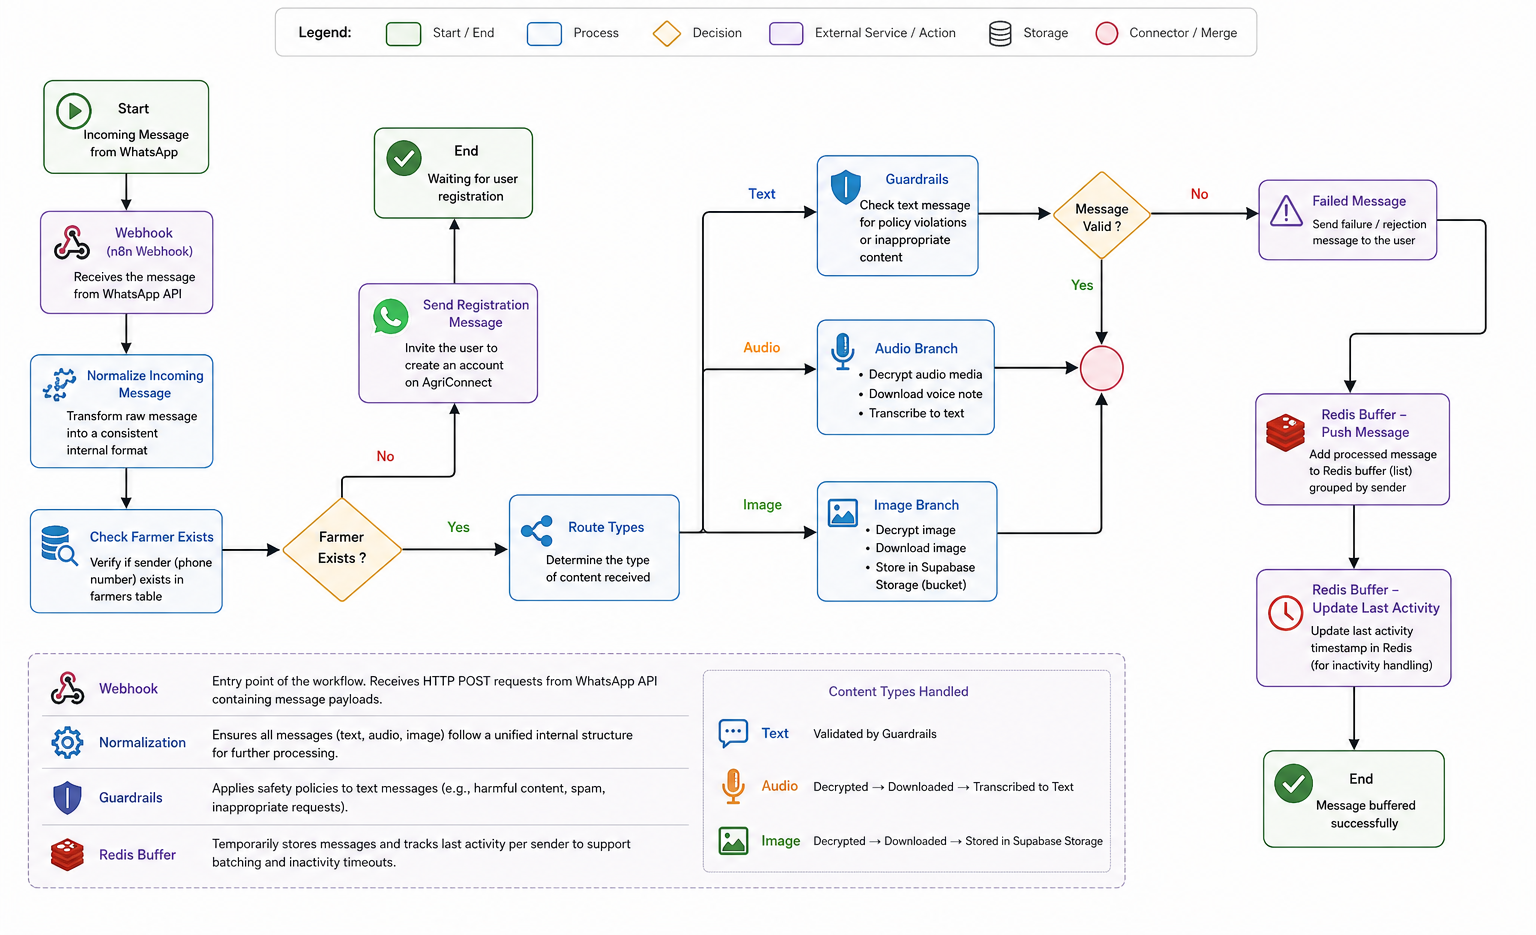
\includegraphics[width=\textwidth]{images/diagrammes/W00_flowchart.png}
    \caption{W00 — Message Reception Workflow}
    \label{fig:w00-workflow}
\end{figure}

\subsection{W01 — Orchestrator Workflow}

W01 is the central processing pipeline, triggered every five seconds. It scans Redis buffers for completed conversations, performs visual preanalysis when an image is present, normalizes the batch via the Normalizer Agent, and passes the result to the Orchestrator Agent, which selectively invokes sub-agents and routes the final response back to the farmer as text or audio. The full implementation is detailed in the realization chapter.

\begin{figure}[H]
    \centering
    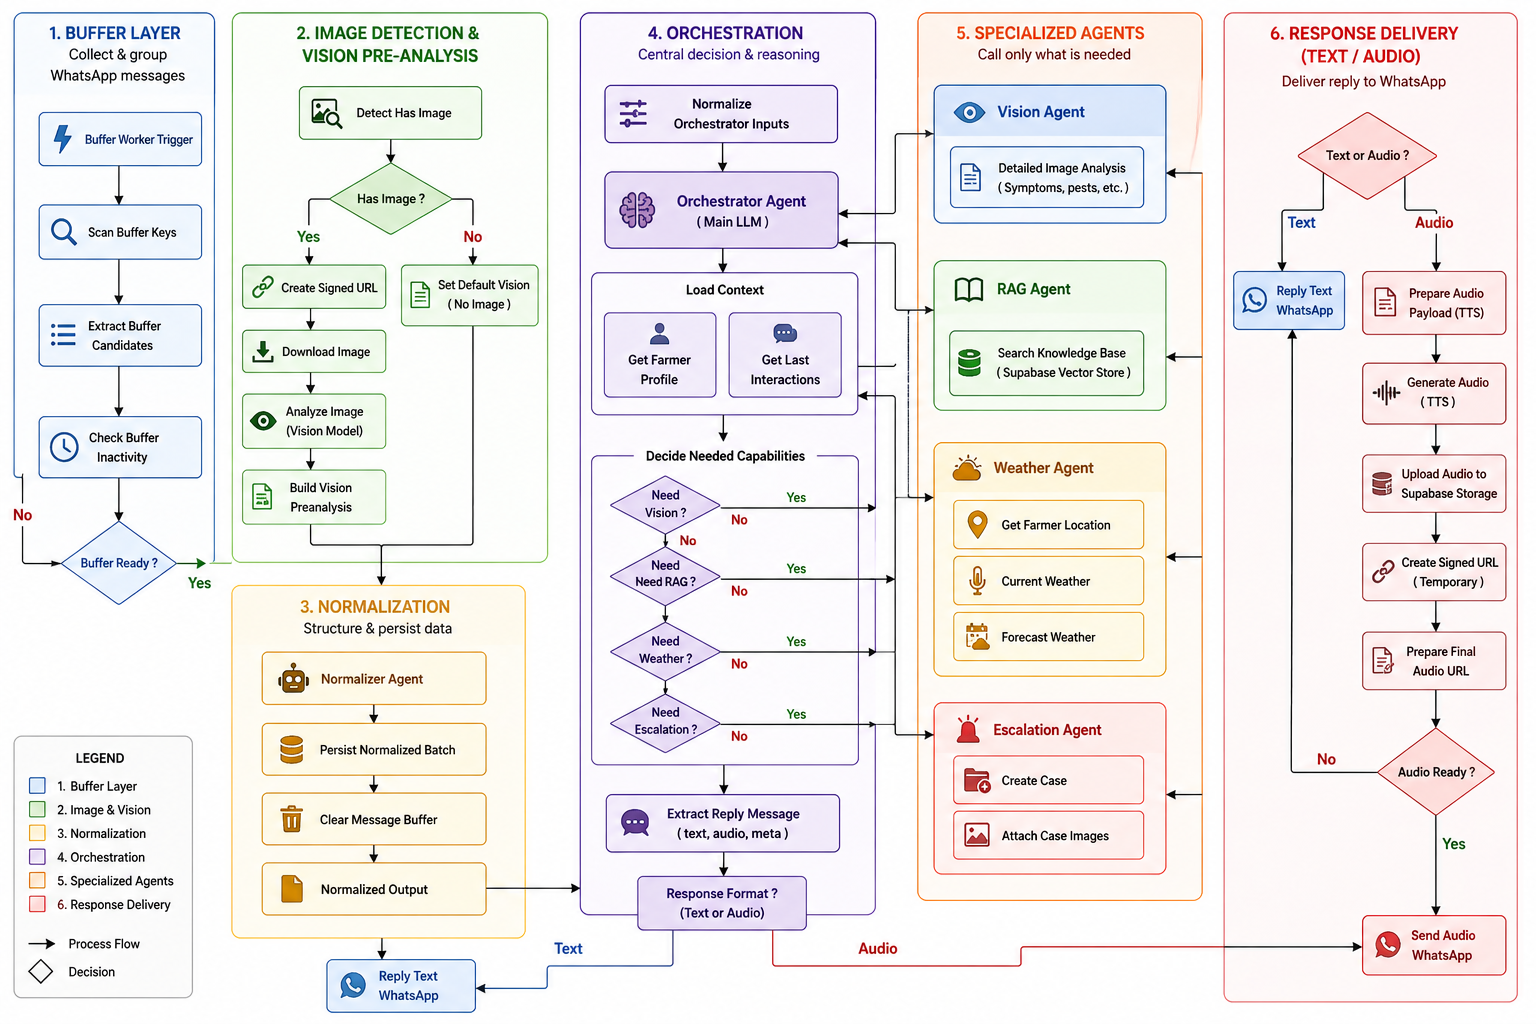
\includegraphics[width=\textwidth]{images/diagrammes/W01_ORCHESTRATOR.png}
    \caption{W01 — Orchestrator Workflow}
    \label{fig:w01-workflow}
\end{figure}

\subsection{Vision Sub-Workflow}

The Vision Sub-Workflow is invoked by the Orchestrator Agent when a crop image passes the preanalysis quality gate. It submits the image in parallel to four PlantNet API endpoints (species, flora, disease, variety) and returns a merged structured output with ranked candidates and confidence scores to the orchestrator.

\begin{figure}[H]
    \centering
    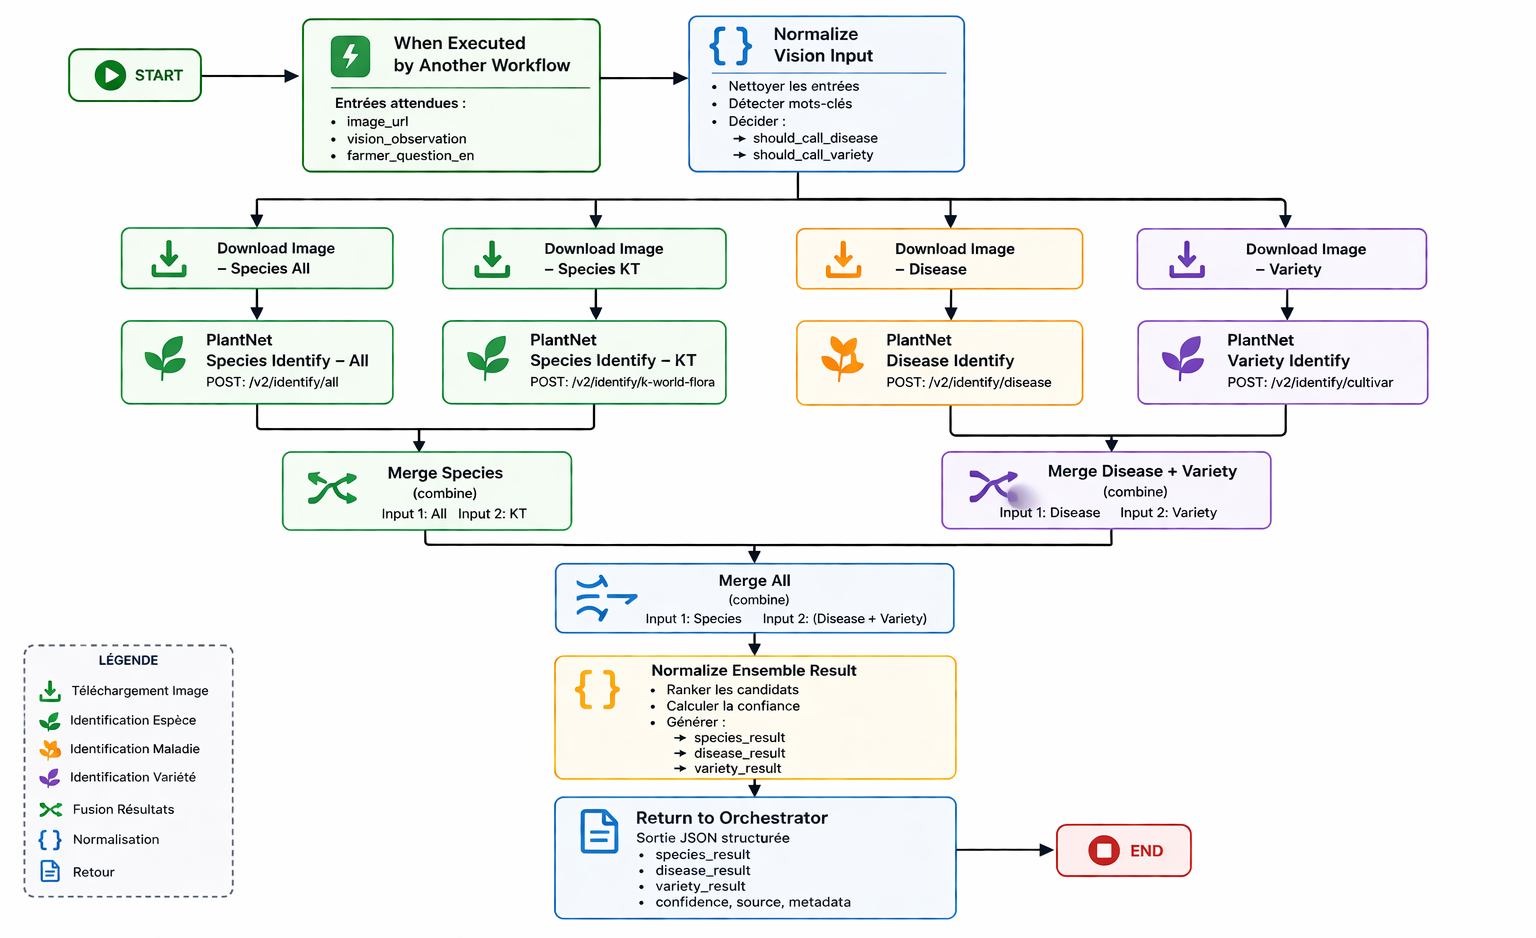
\includegraphics[width=\textwidth]{images/diagrammes/W02_VISION.png}
    \caption{Vision Sub-Workflow — Parallel PlantNet Analysis}
    \label{fig:vision-workflow}
\end{figure}

\subsection{KB Ingestion Workflow}

The KB Ingestion Workflow maintains the agricultural knowledge base autonomously. Triggered by a Google Drive event, it deduplicates the file, removes outdated chunks from the Supabase vector store, downloads and chunks the new document, embeds the chunks using OpenAI embeddings, and notifies the administrator by email upon completion.

\section{Database Design}

The database design of the AgriConnect system aims to ensure efficient storage, consistency, and retrieval of data related to users, agricultural cases, and interactions between different actors. The system relies on a relational database model organized into multiple schemas, allowing modularity, scalability, and clear separation of concerns.

The system uses \textbf{Supabase}, built on PostgreSQL, as the primary database engine. Structured data is stored in relational tables, media files (images, audio, avatars) are stored in Supabase Storage buckets, and vector embeddings are stored in a pgvector-enabled \texttt{documents} table for semantic retrieval.

The database is organized around a \textit{core} schema containing the main operational entities. The \textit{users} table is the central entity, extended by \textit{farmers} and \textit{agronomists} tables with role-specific attributes, and a \textit{locations} table for geographical data. Case management is handled by the \textit{cases}, \textit{proposals}, \textit{feedback}, and \textit{case\_images} tables. Referential integrity is enforced through UUID primary keys, foreign key constraints, and enumerated types for status, priority, and proposal lifecycle values.

\begin{figure}[H]
    \centering
    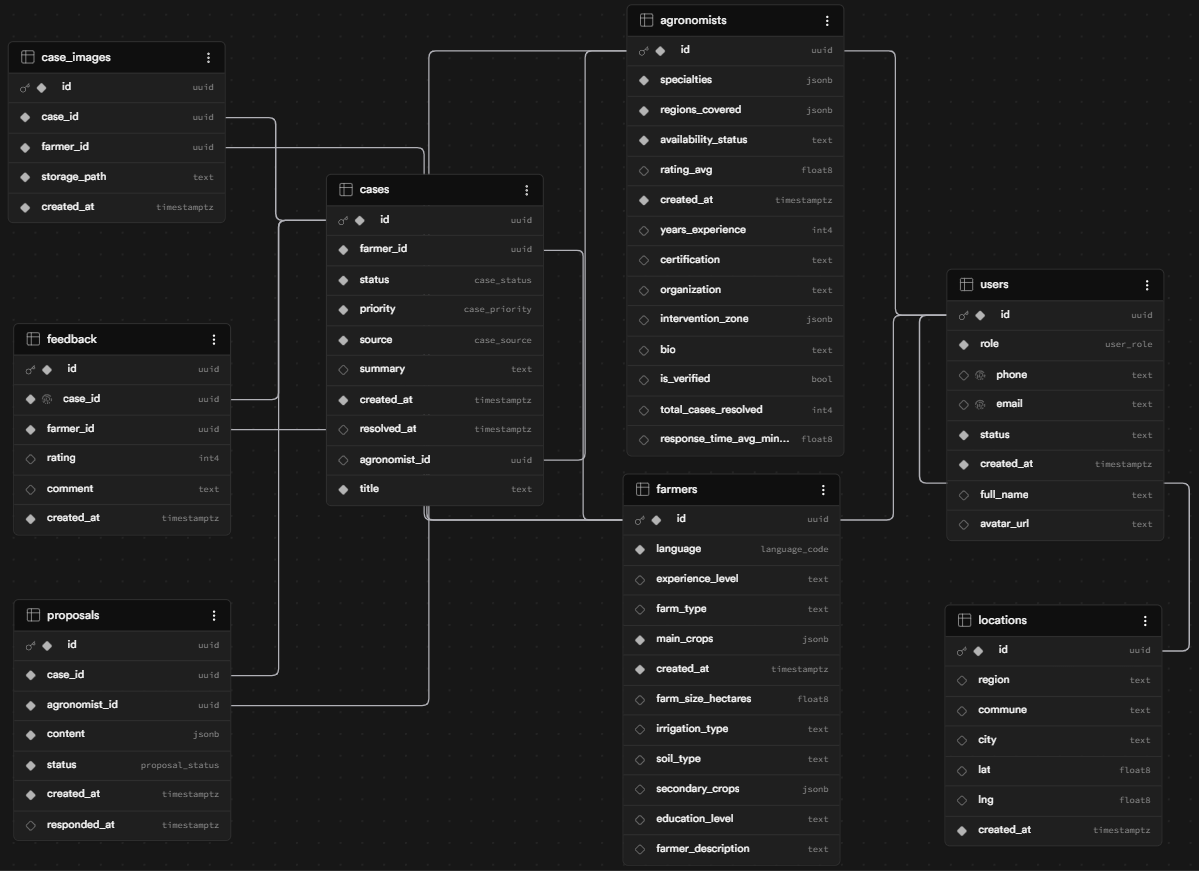
\includegraphics[width=\textwidth]{images/database/core_schema.png}
    \caption{Core Schema Structure}
    \label{fig:core_schema}
\end{figure}
\section{Orchestration Strategy}

The orchestration strategy of AgriConnect is based on a dynamic, context-driven agent invocation model rather than a fixed sequential pipeline. The Orchestrator Agent does not invoke all specialized agents for every interaction; instead, it evaluates the normalized input and applies a set of explicit rules to determine which agents are necessary for the current request.

Agent activation follows a defined priority order. The orchestrator always begins by loading the farmer profile and recent interaction history before any other reasoning. Vision Agent invocation is conditional on the presence of a usable image that passed the preanalysis quality gate. RAG Agent invocation is conditional on a non-ambiguous, agronomically relevant query being resolvable from text or image evidence. Weather Agent invocation is limited to requests where environmental conditions materially affect timing or field action decisions. Escalation Agent invocation is reserved for urgent, unresolved, or high-risk situations that exceed the system’s automated reasoning capacity.

This selective invocation strategy reduces unnecessary API calls, improves response latency for simple requests, and ensures that each agent is only called with complete and valid inputs. Each agent operates under a strict output contract defined by a JSON schema, which the orchestrator uses to fuse results conservatively and produce a final reply that reflects only what the available evidence supports.

\section{Context Management and Personalization}

AgriConnect maintains conversational context and personalizes responses through three complementary mechanisms integrated into the Orchestrator Agent.

The first mechanism is the \textbf{PostgreSQL conversation memory}, which stores the last twenty turns of each farmer’s conversation indexed by phone number. This memory allows the orchestrator to recognize follow-up messages, resolve ambiguous references to previous topics, and avoid asking clarification questions that the farmer has already answered in the same session.

The second mechanism is \textbf{farmer profile retrieval}. At each orchestration step, the system queries the \texttt{v\_farmer\_context} view to load the farmer’s preferred language, experience level, farm type, main crops, and geographical location. This profile data informs the reply language selection, the level of technical detail in the response, and the location parameter passed to the Weather Agent.

The third mechanism is \textbf{recent interaction history}, which provides the last twenty interaction records from the database. This history allows the orchestrator to detect recurring unresolved issues, identify the most recent topic discussed, and determine whether the current message is a continuation of an ongoing agronomic case or a new independent request.

Together, these mechanisms ensure that farmers receive responses that are adapted to their profile, consistent with the ongoing conversation, and sensitive to the cumulative context of their past interactions with the platform.

\section{Conclusion}

This chapter presented the complete design of the AgriConnect system, translating the requirements identified in the previous chapter into a structured and coherent architecture.

The overall system architecture was organized into five layers — client, integration, workflow, data, and external services — providing a clear separation of concerns between user-facing interfaces, internal processing logic, persistent storage, and third-party dependencies.

The multi-agent system design described how a central Orchestrator Agent coordinates four specialized agents — RAG, Vision, Weather, and Escalation — each operating under a strict output contract and invoked selectively based on the nature of the incoming request.

UML modeling described the system from three complementary perspectives: the use case diagram captured the functional responsibilities of each actor, the class diagram defined the structural organization of the main data entities, and the state machine diagram formalized the lifecycle of agricultural cases from creation to closure.

The workflow design detailed the four n8n workflows that implement the system: the Message Reception workflow handles incoming WhatsApp events and populates the Redis buffer; the Orchestrator workflow manages buffer processing, visual preanalysis, normalization, agent coordination, and response delivery; the Vision Sub-Workflow performs parallel PlantNet-based crop image analysis; and the KB Ingestion workflow autonomously maintains the agricultural knowledge base from Google Drive.

The database design defined a layered storage architecture combining a PostgreSQL relational schema, a Supabase vector store for semantic retrieval, and object storage for binary media. The orchestration strategy and context management sections completed the design by describing how agent invocation is controlled dynamically and how conversational continuity and personalization are maintained across turns.

Overall, this design establishes a solid and verifiable foundation for the implementation phase, in which each described component will be realized and validated in practice.
